% ==============================================================================
% CHƯƠNG 4: CÀI ĐẶT VÀ TRIỂN KHAI
% ==============================================================================

\chapter{CÀI ĐẶT VÀ TRIỂN KHAI}
\label{chap:implementation}

Chương này trình bày chi tiết quá trình cài đặt và triển khai hệ thống, từ việc chuẩn bị môi trường phát triển, thu thập dữ liệu huấn luyện, đến việc đóng gói sản phẩm cuối cùng. Các kết quả đánh giá chi tiết sẽ được trình bày ở Chương~\ref{chap:results}.

\section{Môi trường phát triển}

\subsection{Yêu cầu phần cứng}

\begin{table}[H]
\centering
\caption{Cấu hình phần cứng khuyến nghị}
\label{tab:hardware}
\begin{tabular}{@{}lll@{}}
\toprule
\textbf{Thành phần} & \textbf{Tối thiểu} & \textbf{Khuyến nghị} \\
\midrule
CPU & Intel Core i5 / AMD Ryzen 5 & Intel Core i7 / AMD Ryzen 7 \\
RAM & 8 GB & 16 GB \\
GPU & Tích hợp (iGPU) & NVIDIA GTX 1650 trở lên \\
Webcam & 720p & 1080p \\
Storage & 5 GB SSD & 10 GB SSD \\
\bottomrule
\end{tabular}
\end{table}

\subsection{Yêu cầu phần mềm}

\begin{table}[H]
\centering
\caption{Các thư viện Python sử dụng}
\label{tab:requirements}
\begin{tabular}{@{}llp{6cm}@{}}
\toprule
\textbf{Thư viện} & \textbf{Phiên bản} & \textbf{Mục đích} \\
\midrule
Python & $\geq$ 3.9 & Ngôn ngữ lập trình chính \\
opencv-python & $\geq$ 4.8.0 & Xử lý ảnh và video \\
numpy & $\geq$ 1.24.0 & Tính toán ma trận \\
pillow & $\geq$ 10.0.0 & Vẽ text Unicode \\
customtkinter & $\geq$ 5.2.0 & Giao diện người dùng \\
ultralytics & $\geq$ 8.0.0 & YOLO framework \\
torch & (tự động) & Backend deep learning \\
kaggle & $\geq$ 1.6.0 & Tải dataset \\
pytest & $\geq$ 7.0 & Unit testing \\
\bottomrule
\end{tabular}
\end{table}

\section{Cấu trúc dự án}

Mã nguồn được tổ chức theo cấu trúc module hóa rõ ràng:

\begin{lstlisting}[language=bash,caption={Cấu trúc thư mục dự án},label={lst:project_structure}]
banana-quality-grading/
|-- main.py                  # Entry point
|-- requirements.txt         # Dependencies
|-- training_script.py       # Train detector
|-- training_kaggle_classification.py  # Train classifier
|-- export_android_models.py # Export TFLite
|
|-- app/
|   |-- __init__.py
|   |-- banana_analyzer.py   # Feature extraction module
|   |-- grader.py            # Main grading logic
|   |-- text_overlay.py      # Vietnamese text rendering
|   |-- ui_manager.py        # CustomTkinter UI
|   |-- video_thread.py      # Capture & threading
|
|-- utils/
|   |-- resource_manager.py  # Auto-download resources
|
|-- weights/
|   |-- best.pt              # Classifier weights
|   |-- detector.pt          # Custom detector (optional)
|
|-- datasets/
|   |-- kaggle_banana_ripeness/  # Kaggle dataset
|
|-- runs_banana/             # Training outputs
|   |-- yolov8n_banana_cls/
|       |-- weights/best.pt
|
|-- tests/                   # Unit tests
    |-- test_grader_real_model_integration.py
\end{lstlisting}

\section{Huấn luyện mô hình}

\subsection{Dataset}

\subsubsection{Nguồn gốc và đặc điểm dữ liệu}

Chúng tôi sử dụng tập dữ liệu \textbf{Banana Classification Dataset} từ Kaggle \ref{ref:kaggle_banana_classification}, một dataset được xây dựng với mục đích huấn luyện các mô hình học máy phát hiện và phân loại chất lượng chuối. Điểm đặc biệt của dataset này là nó được tổng hợp từ dự án \textbf{Banana Ripeness Classification} trên nền tảng Roboflow Universe \ref{ref:roboflow_banana}, đảm bảo tính đa dạng và chất lượng annotation.

\begin{table}[H]
\centering
\caption{Thống kê chi tiết Banana Classification Dataset}
\label{tab:dataset_stats}
\begin{tabular}{@{}llr@{}}
\toprule
\textbf{Thuộc tính} & \textbf{Mô tả} & \textbf{Giá trị} \\
\midrule
\multicolumn{3}{@{}l}{\textit{Tổng quan}} \\
\midrule
Tổng số ảnh & Toàn bộ dataset & 13,500 ảnh \\
Kích thước dataset & Dung lượng lưu trữ & 227.18 MB \\
Giấy phép & Open source & MIT License \\
\midrule
\multicolumn{3}{@{}l}{\textit{Phân chia dữ liệu}} \\
\midrule
Training set & Dùng để huấn luyện & $\sim$10,800 ảnh (80\%) \\
Validation set & Đánh giá trong quá trình train & $\sim$1,350 ảnh (10\%) \\
Test set & Đánh giá cuối cùng & $\sim$1,350 ảnh (10\%) \\
\midrule
\multicolumn{3}{@{}l}{\textit{Phân bố các lớp}} \\
\midrule
Unripe (Xanh) & Chuối còn xanh, chưa chín & $\sim$3,375 ảnh \\
Ripe (Chín) & Chuối chín vàng, chất lượng tốt & $\sim$3,375 ảnh \\
Overripe (Quá chín) & Chuối có đốm nâu, bắt đầu mềm & $\sim$3,375 ảnh \\
Rotten (Thối) & Chuối hỏng, không sử dụng được & $\sim$3,375 ảnh \\
\bottomrule
\end{tabular}
\end{table}

\subsubsection{Phân tích chất lượng dữ liệu}

Từ góc nhìn của một nhà nghiên cứu, việc lựa chọn dataset không chỉ dừng lại ở số lượng mà còn phải xem xét kỹ lưỡng về \textit{chất lượng} và \textit{tính đại diện} của dữ liệu. Dataset này có một số điểm mạnh và hạn chế đáng lưu ý:

\textbf{Điểm mạnh:}
\begin{itemize}
    \item \textbf{Cân bằng giữa các lớp}: Phân bố đều giữa 4 class giúp tránh bias trong quá trình training.
    \item \textbf{Đa dạng điều kiện chụp}: Ảnh được thu thập từ nhiều nguồn, với các điều kiện ánh sáng và góc độ khác nhau.
    \item \textbf{Annotation rõ ràng}: Ranh giới giữa các class được định nghĩa tương đối rõ ràng dựa trên đặc điểm thị giác.
\end{itemize}

\textbf{Hạn chế cần lưu ý:}
\begin{itemize}
    \item \textbf{Không có bounding box annotation}: Dataset chỉ hỗ trợ classification, không có object detection labels. Đây chính là constraint cơ bản dẫn đến quyết định thiết kế pipeline 2 giai đoạn.
    \item \textbf{Nền ảnh đơn giản}: Phần lớn ảnh có nền trắng hoặc đơn sắc, có thể ảnh hưởng đến khả năng tổng quát hóa khi deploy trong môi trường thực tế.
    \item \textbf{Chủ yếu chuối Cavendish}: Dataset tập trung vào giống chuối tiêu, có thể không tổng quát hóa tốt sang các giống chuối địa phương Việt Nam.
\end{itemize}

\subsubsection{Lý do lựa chọn dataset}

Việc lựa chọn Banana Classification Dataset từ Kaggle xuất phát từ những suy xét mang tính phương pháp luận:

\begin{enumerate}
    \item \textbf{Tính mở và tái tạo được}: Dataset có giấy phép MIT, cho phép sử dụng cho mục đích học thuật và thương mại.
    
    \item \textbf{Kích thước phù hợp}: $\sim$13,500 ảnh đủ lớn để fine-tune một classifier từ pretrained weights, nhưng không quá lớn gây khó khăn về tài nguyên tính toán.
    
    \item \textbf{Cấu trúc chuẩn}: Định dạng folder-per-class tương thích trực tiếp với Ultralytics YOLO classification pipeline, giảm thiểu công sức tiền xử lý.
    
    \item \textbf{Cộng đồng hỗ trợ}: Dataset có hơn 2,000 lượt tải và nhiều notebooks tham khảo trên Kaggle, cho phép benchmark và so sánh kết quả.
\end{enumerate}

\subsection{Quy trình huấn luyện Classifier}

\begin{lstlisting}[language=bash,caption={Lệnh huấn luyện classifier},label={lst:train_cmd}]
# Buoc 1: Cau hinh Kaggle API
# Dat kaggle.json tai: %USERPROFILE%/.kaggle/kaggle.json

# Buoc 2: Chay script train (tu dong download dataset)
python training_kaggle_classification.py \
    --device auto \
    --epochs 50 \
    --imgsz 416 \
    --batch -1

# Buoc 3: Copy weights
copy runs_banana\yolov8n_banana_cls\weights\best.pt weights\best.pt
\end{lstlisting}

\subsection{Cấu hình huấn luyện}

\begin{table}[H]
\centering
\caption{Tham số huấn luyện classifier}
\label{tab:train_config}
\begin{tabular}{@{}ll@{}}
\toprule
\textbf{Tham số} & \textbf{Giá trị} \\
\midrule
Base model & yolov8n-cls.pt (pretrained ImageNet) \\
Image size & 416 $\times$ 416 \\
Epochs & 50 \\
Batch size & Auto (-1) \\
Optimizer & Auto (AdamW) \\
Learning rate & Auto-tuned \\
Device & GPU (CUDA) nếu có, ngược lại CPU \\
Augmentation & Default Ultralytics (flip, scale, HSV) \\
\bottomrule
\end{tabular}
\end{table}

\subsection{Kết quả huấn luyện}

Dựa trên file \texttt{results.csv} từ run \texttt{yolov8n\_banana\_cls3}:

\begin{table}[H]
\centering
\caption{Kết quả huấn luyện qua các epoch}
\label{tab:train_results}
\begin{tabular}{@{}ccccc@{}}
\toprule
\textbf{Epoch} & \textbf{Train Loss} & \textbf{Val Loss} & \textbf{Top-1 Acc} & \textbf{Top-5 Acc} \\
\midrule
1 & 0.6867 & 0.1191 & 96.35\% & 100\% \\
10 & 0.0537 & 0.0933 & 97.33\% & 100\% \\
20 & 0.0326 & 0.0623 & 98.66\% & 100\% \\
30 & 0.0218 & 0.1002 & 98.40\% & 100\% \\
40 & 0.0173 & 0.0638 & 98.66\% & 100\% \\
50 & 0.0096 & 0.0752 & 98.75\% & 100\% \\
\bottomrule
\end{tabular}
\end{table}

\begin{figure}[H]
\centering
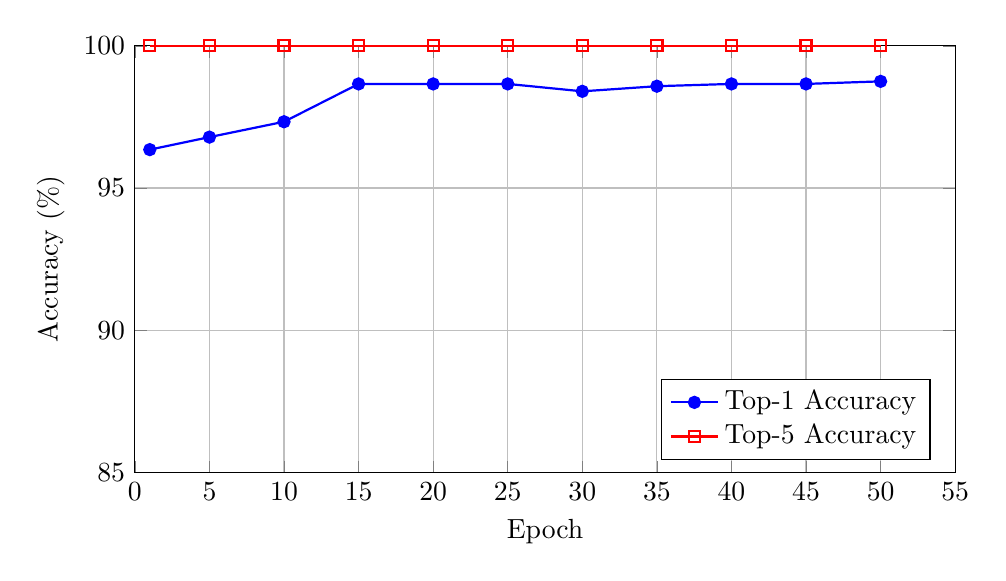
\begin{tikzpicture}
\begin{axis}[
    xlabel={Epoch},
    ylabel={Accuracy (\%)},
    xmin=0, xmax=55,
    ymin=85, ymax=100,
    legend pos=south east,
    grid=major,
    width=12cm,
    height=7cm
]
\addplot[blue, thick, mark=*] coordinates {
    (1, 96.35) (5, 96.79) (10, 97.33) (15, 98.66) (20, 98.66)
    (25, 98.66) (30, 98.40) (35, 98.58) (40, 98.66) (45, 98.66) (50, 98.75)
};
\addlegendentry{Top-1 Accuracy}

\addplot[red, thick, mark=square] coordinates {
    (1, 100) (5, 100) (10, 100) (15, 100) (20, 100)
    (25, 100) (30, 100) (35, 100) (40, 100) (45, 100) (50, 100)
};
\addlegendentry{Top-5 Accuracy}
\end{axis}
\end{tikzpicture}
\caption{Biểu đồ accuracy qua quá trình huấn luyện}
\label{fig:train_curve}
\end{figure}

\textbf{Nhận xét sơ bộ:} Model hội tụ nhanh, đạt $>97\%$ Top-1 accuracy sau 10 epoch. Phân tích chi tiết về learning curve, confusion matrix và error pattern sẽ được trình bày ở Chương~\ref{chap:results}.

\begin{figure}[H]
\centering
\begin{subfigure}[b]{0.32\textwidth}
    \includegraphics[width=\textwidth]{images/train_batch0.jpg}
    \caption{Training batch 0}
\end{subfigure}
\hfill
\begin{subfigure}[b]{0.32\textwidth}
    \includegraphics[width=\textwidth]{images/train_batch1.jpg}
    \caption{Training batch 1}
\end{subfigure}
\hfill
\begin{subfigure}[b]{0.32\textwidth}
    \includegraphics[width=\textwidth]{images/train_batch2.jpg}
    \caption{Training batch 2}
\end{subfigure}
\caption{Một số batch dữ liệu huấn luyện đã qua augmentation. Các ảnh được tự động scale, flip và điều chỉnh màu sắc bởi Ultralytics pipeline, giúp tăng tính đa dạng và khả năng tổng quát hóa của mô hình.}
\label{fig:train_batches}
\end{figure}

\section{Phát triển giao diện người dùng}

\subsection{Thiết kế UI}

Giao diện được xây dựng bằng \textbf{CustomTkinter} --- thư viện mở rộng Tkinter với giao diện dark mode hiện đại.

\begin{figure}[H]
\centering
\includegraphics[width=0.9\textwidth]{images/screen.PNG}
\caption{Giao diện chính của ứng dụng}
\label{fig:ui_screenshot}
\end{figure}

\subsection{Các thành phần giao diện}

\begin{table}[H]
\centering
\caption{Mô tả các thành phần UI}
\label{tab:ui_components}
\begin{tabular}{@{}lp{8cm}@{}}
\toprule
\textbf{Thành phần} & \textbf{Chức năng} \\
\midrule
Video Panel & Hiển thị luồng webcam với bbox overlay và label \\
Status Label & Trạng thái hiện tại: ``Đang quay'', ``Đã dừng'', lỗi \\
Grade Label & Kết quả phân loại: ``Chuối Xanh'', ``Chín Vừa'', v.v. \\
Confidence Label & Độ tin cậy của classifier (\%) \\
FPS Label & Tốc độ xử lý hiện tại \\
Quality Panel & Thông tin chi tiết: điểm chất lượng, màu sắc, số đốm \\
Start/Stop Button & Bật/tắt camera \\
\bottomrule
\end{tabular}
\end{table}

\subsection{Hỗ trợ tiếng Việt}

OpenCV \texttt{cv2.putText()} không hỗ trợ Unicode tiếng Việt tốt. Chúng tôi giải quyết bằng cách sử dụng Pillow:

\begin{lstlisting}[caption={Vẽ text tiếng Việt bằng Pillow},label={lst:vietnamese_text}]
class UnicodeTextRenderer:
    def draw_label(self, frame_bgr, text_vi, text_en, xy, color_bgr):
        font = self._load_font()
        
        if font is None:
            # Fallback sang English với OpenCV
            cv2.putText(frame_bgr, text_en, xy, 
                       cv2.FONT_HERSHEY_SIMPLEX, 0.6, color_bgr, 2)
            return frame_bgr
        
        # PIL rendering (ho tro Unicode)
        frame_rgb = cv2.cvtColor(frame_bgr, cv2.COLOR_BGR2RGB)
        pil_img = Image.fromarray(frame_rgb)
        draw = ImageDraw.Draw(pil_img)
        
        # Ve background rounded rectangle
        draw.rounded_rectangle(...)
        
        # Ve text tieng Viet
        draw.text((x, y), text_vi, font=font, fill=color_rgb)
        
        return cv2.cvtColor(np.array(pil_img), cv2.COLOR_RGB2BGR)
\end{lstlisting}

\section{Tích hợp và kiểm thử}

\subsection{Unit Testing}

Dự án sử dụng \texttt{pytest} cho unit testing:

\begin{lstlisting}[language=bash,caption={Chạy test},label={lst:run_tests}]
# Chay tat ca test
pytest tests/ -v

# Chay test voi coverage report
pytest tests/ --cov=app --cov-report=html
\end{lstlisting}

\subsection{Test với mô hình thực}

File \texttt{test\_grader\_real\_model\_integration.py} thực hiện integration test với model thực:

\begin{itemize}
    \item Load model từ \texttt{weights/best.pt}
    \item Chạy inference trên ảnh test
    \item Kiểm tra output có đúng format
    \item Ghi artifact (ảnh annotated + JSON) để debug
\end{itemize}

\section{Triển khai và đóng gói}

\subsection{Chạy ứng dụng}

\begin{lstlisting}[language=bash,caption={Các bước chạy ứng dụng},label={lst:run_app}]
# 1. Tao virtual environment
python -m venv .venv
.\.venv\Scripts\activate

# 2. Cai dat dependencies
pip install -r requirements.txt

# 3. Kiem tra setup
python check_setup.py

# 4. Chay ung dung
python main.py
\end{lstlisting}

\subsection{Export cho Android (TFLite)}

Hệ thống hỗ trợ export model sang TensorFlow Lite để chạy trên Android:

\begin{lstlisting}[language=bash,caption={Export TFLite},label={lst:export_tflite}]
python export_android_models.py \
    --classifier weights/best.pt \
    --detector yolov8n.pt \
    --imgsz 416

# Output: exports_android/
#   - classifier.tflite
#   - detector.tflite
\end{lstlisting}

\subsection{Build executable (Windows)}

Script \texttt{build\_exe.ps1} sử dụng PyInstaller để đóng gói thành file .exe độc lập:

\begin{lstlisting}[language=bash,caption={Build executable},label={lst:build_exe}]
# Chay PowerShell script
.\build_exe.ps1

# Output: dist/banana_quality_grading.exe
\end{lstlisting}

\section{Biến môi trường cấu hình}

\begin{table}[H]
\centering
\caption{Các biến môi trường hỗ trợ}
\label{tab:env_vars}
\begin{tabular}{@{}llp{5cm}@{}}
\toprule
\textbf{Biến} & \textbf{Mặc định} & \textbf{Mô tả} \\
\midrule
BANANA\_DEVICE & auto & Device inference: cpu, 0, auto \\
BANANA\_DETECTOR\_PATH & (auto) & Đường dẫn detector weights \\
BANANA\_DETECTOR\_BACKEND & yolo & yolo hoặc haar \\
BANANA\_HAAR\_PATH & haarbanana.xml & Đường dẫn Haar cascade \\
BANANA\_MAX\_FRUITS & 6 & Số quả tối đa/frame \\
BANANA\_DET\_IMGSZ & 640 & Kích thước input detector \\
BANANA\_CLS\_IMGSZ & 416 & Kích thước input classifier \\
BANANA\_BBOX\_HOLD & 5 & Số frame giữ bbox \\
BANANA\_MODEL\_URL & (empty) & URL tải weights tự động \\
BANANA\_FONT\_URL & (empty) & URL tải font tự động \\
\bottomrule
\end{tabular}
\end{table}

\section{Tóm tắt chương}

Chương này đã trình bày chi tiết quá trình cài đặt và triển khai hệ thống phân loại chất lượng chuối, bao gồm:
\begin{itemize}
    \item Thiết lập môi trường phát triển và các thư viện cần thiết.
    \item Thu thập và phân tích dữ liệu huấn luyện từ Kaggle.
    \item Quy trình huấn luyện classifier với các tham số tối ưu.
    \item Phát triển giao diện người dùng hỗ trợ tiếng Việt.
    \item Kiểm thử và đóng gói sản phẩm.
\end{itemize}

Với nền tảng kỹ thuật đã được thiết lập, chương tiếp theo sẽ đi sâu vào \textbf{đánh giá kết quả} --- phân tích hiệu năng của cả model ``thô'' (classifier) lẫn pipeline hoàn chỉnh trên dữ liệu thực tế.

\clearpage
